\documentclass{article} % For LaTeX2e
\usepackage{nips15submit_e,times}
\usepackage{hyperref}
\usepackage{url}
\usepackage{graphicx}
%\documentstyle[nips14submit_09,times,art10]{article} % For LaTeX 2.09

\title{EEG curiosities}

\author{
Manuel Nickel
\\
%Technische Universit\"at M\"unchen\\
%Pittsburgh, PA 15213 \\
\texttt{manuel.nickel@tum.de} \\
\And
Dominik Irimi \\
%Affiliation \\
%Address \\
\texttt{dominik.irimi@gmail.com} \\
\AND
Christoph Dehner \\
%Affiliation \\
%Address \\
\texttt{dehner@in.tum.de} \\
\And
Roman C.~Podolski \\
%Affiliation \\
%Address \\
\texttt{roman.podolski@tum.de} \\
\And
Philipp Bergmann \\
%Affiliation \\
%Address \\
\texttt{philipp.bergmann@tum.de} \\
}

% The \author macro works with any number of authors. There are two commands
% used to separate the names and addresses of multiple authors: \And and \AND.
%
% Using \And between authors leaves it to \LaTeX{} to determine where to break
% the lines. Using \AND forces a linebreak at that point. So, if \LaTeX{}
% puts 3 of 4 authors names on the first line, and the last on the second
% line, try using \AND instead of \And before the third author name.

\newcommand{\fix}{\marginpar{FIX}}
\newcommand{\new}{\marginpar{NEW}}

\nipsfinalcopy % Uncomment for camera-ready version

\begin{document}


\maketitle

\begin{abstract}
t-SNE visualizations of parts of the \emph{WAY-EEG-GAL} dataset showed some curious results that were not expected and barely believable. In an attempt to verify the correct function of the implemented algorithm several tests were conducted. The following shall give a review of the results.
\end{abstract}

\section{Introduction}
Using the Barnes Hut t-SNE implementation by L.J.P. van der Maaten a t-SNE plot of all eeg-data points of \emph{Participant 1}, \emph{Series 1} was meant to be made. This data subset of \emph{WAY-EEG-GAL} can be found in \verb|WS_P1_S1.mat|. It includes 34 lifting trials of participant 1's first conducted series and makes up for a total of 146982 data points. t-SNE cannot be able to consider time-relations between individual data points. However, in order to make sure that the used implementation of t-SNE is not somehow influenced by the ordering of the states, all data points were shuffled and placed in random order before being fed to t-SNE. Each of the 34 trials were marked with a different color in the resulting plot, e.g. states of trial 1 might be colored in green while states of trial 2 in red. Furthermore, states that were measured within the time span of the LED being lid up are drawn with a black border in order to separate them visually from states with the LED being off.

Here is what one might expect to see as a result of t-SNE:
\begin{itemize}
	\item The LEDon-states are somewhat grouped together in one place while the LEDoff-states are grouped together in another place:
	This may be considered a sign that it should be possible to extract information about the intention to grasp. As t-SNE does not ``understand'' relations in time even a simple Feedforward Net might work.
	\item All data points are pretty much distributed randomly and there is no apparent structure in the plot:
	This would be a signal that if there is a way to extract information about the intention to grasp, then it is not sufficient to use Feedforward Nets only, but one needs to at least incorporate time relations. Thus, one would try to use Recurrent Neural Nets.
\end{itemize}

\begin{figure}[h]
	\centering
	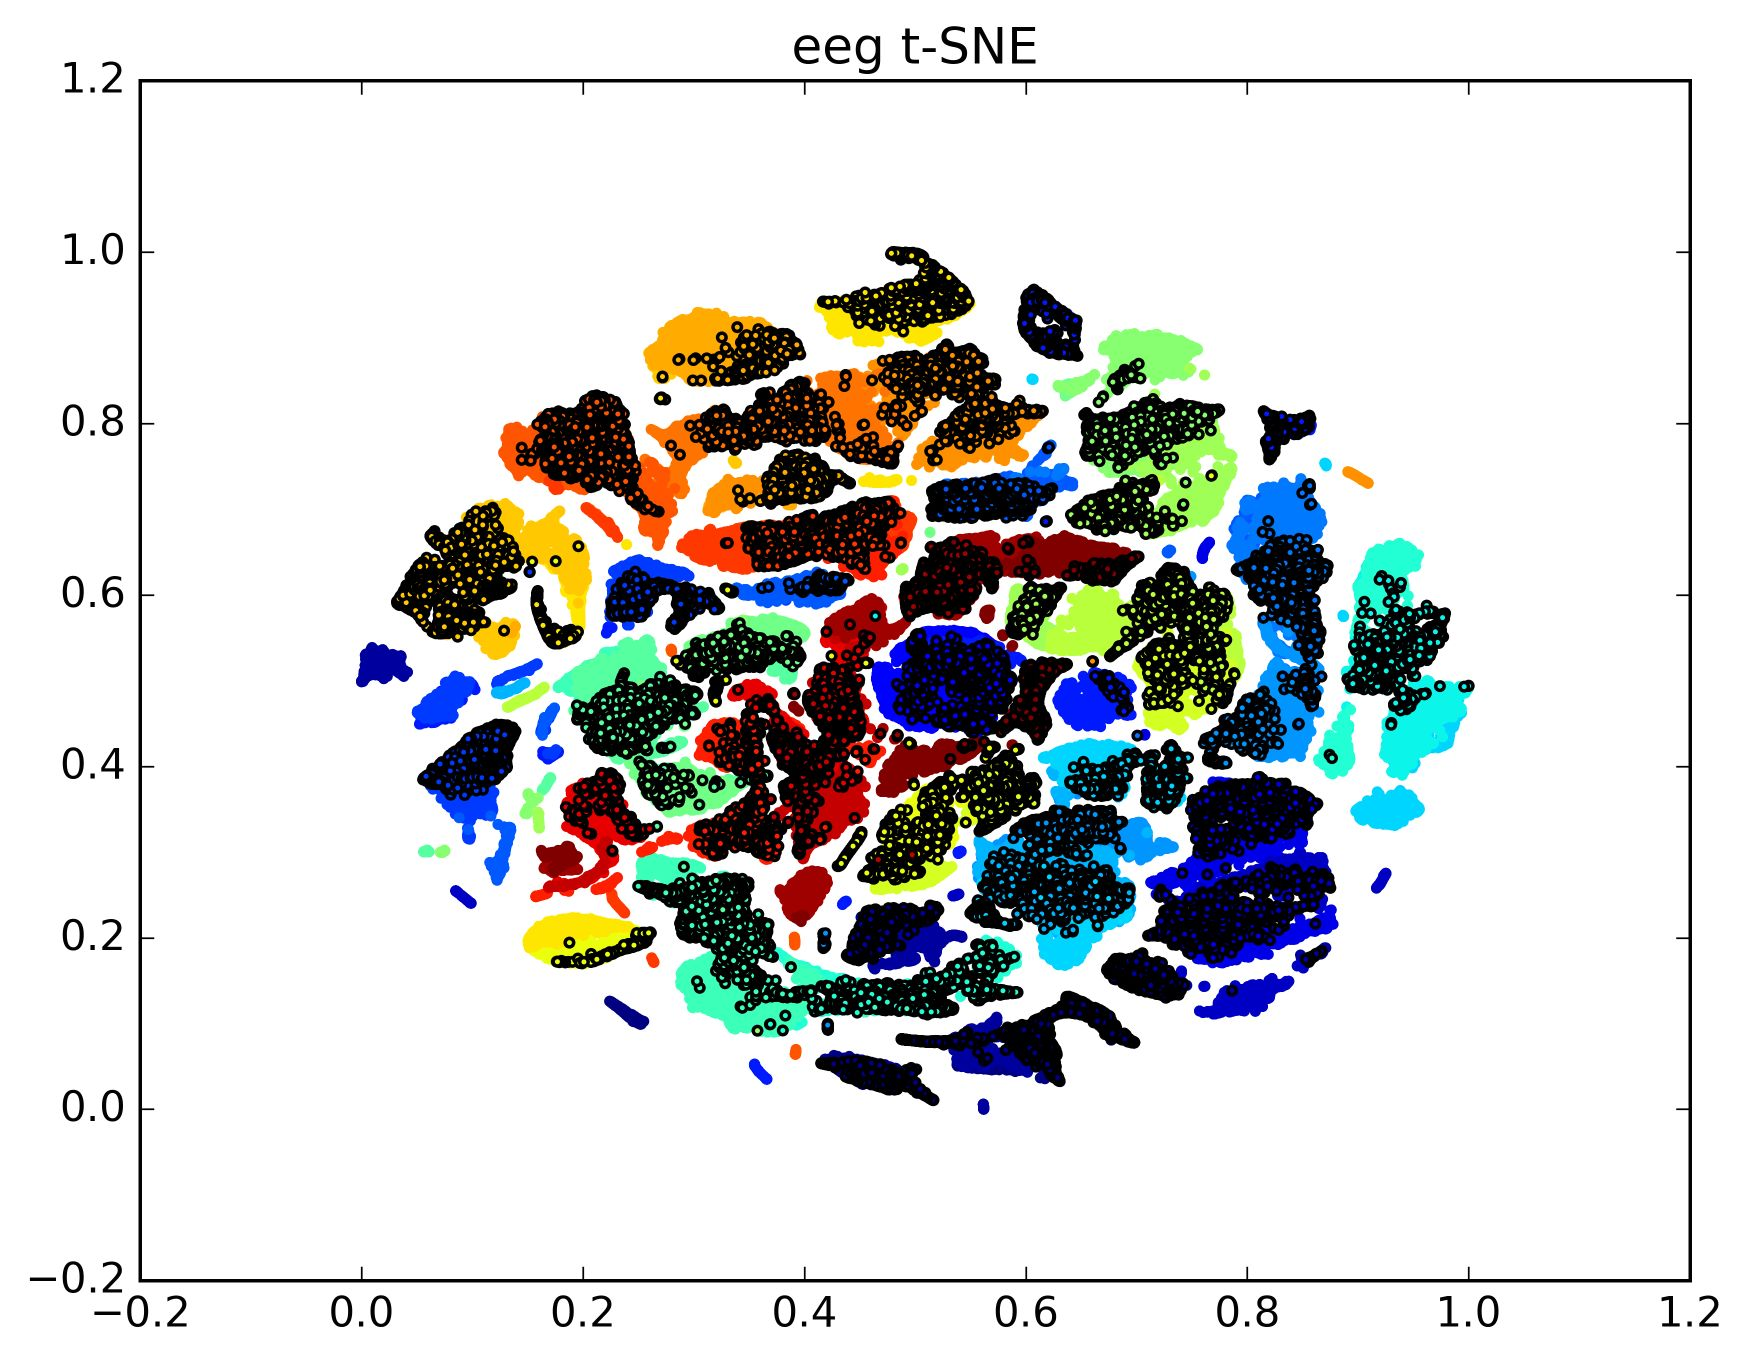
\includegraphics[width=1.0\textwidth]{eeg.jpg}
	\caption{t-SNE plot for 146982 EEG data points}
	\label{fig:eeg}
\end{figure}

However, the actual result of running t-SNE on the provided EEG data is rather surprising. The plot is shown in figure \ref{fig:eeg} and shows clusters of data points that belong to the same trial rather than similar activity like grasping. This indicates that similarities among individual states are rather influenced by during what trial they were produced than what brain activity they might represent.
As this conclusion is rather unbelievable the following steps were conducted to ensure that the used t-SNE implementation in Python is functioning correctly.




\section{Code checking}
The Python code written to apply the EEG data on L.J.P. van der Maaten's Barnes Hut t-SNE algorithm has been checked to work as desired. In particular, key positions within the code were checked multiple times. A debugger was used to view the values of the variable \verb|data_set|, which is given as an argument to \verb|bh_tsne()|, the function that runs the actual algorithm as an executable. These values were compared to those displayed in Matlab verifying that indeed correct data is used. Figure \ref{fig:debug} shows a screenshot of this rather lengthy but trustworthy procedure. These \verb|data_set| values were checked both before randomizing the ordering and after. All checks turned out to be positive.

\begin{figure}[h]
	\centering
	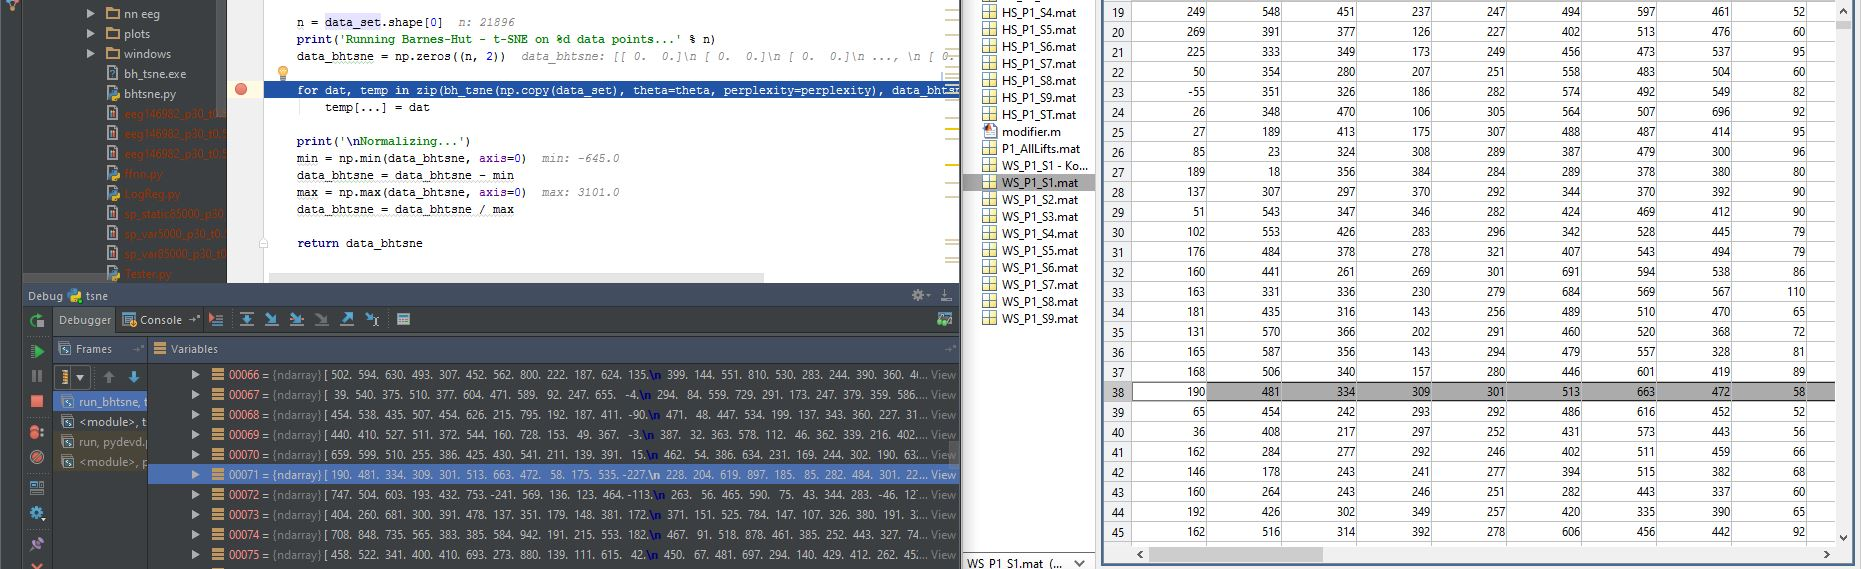
\includegraphics[width=1.0\textwidth]{debug.jpg}
	\caption{Comparing read in EEG values by hand}
	\label{fig:debug}
\end{figure}




\section{Plausibility checks}
In order to make sure that the entire script in combination with L.J.P. van der Maaten's Barnes Hut t-SNE executable gives plausible results in general, several tests were conducted.


\subsection{Running t-SNE on EMG data}
As a first plausibility check the implementation was applied to the EMG data of the same \verb|.mat| file. This data is structured in the same way as EEG, only with a different number of samples per trial and less dimensions. This means that the script can be applied without any changes. If the resulting plot looked like the EEG one, this might hint at some erroneous function within the implementation. However, figure \ref{fig:emg} shows the actual result which looks much like one would expect. For this the data of only 5 trials was used as there about 7 times as many samples per trial compared to EEG and computation time would thus be expected to be about 9 hours.

\begin{figure}[h]
	\centering
	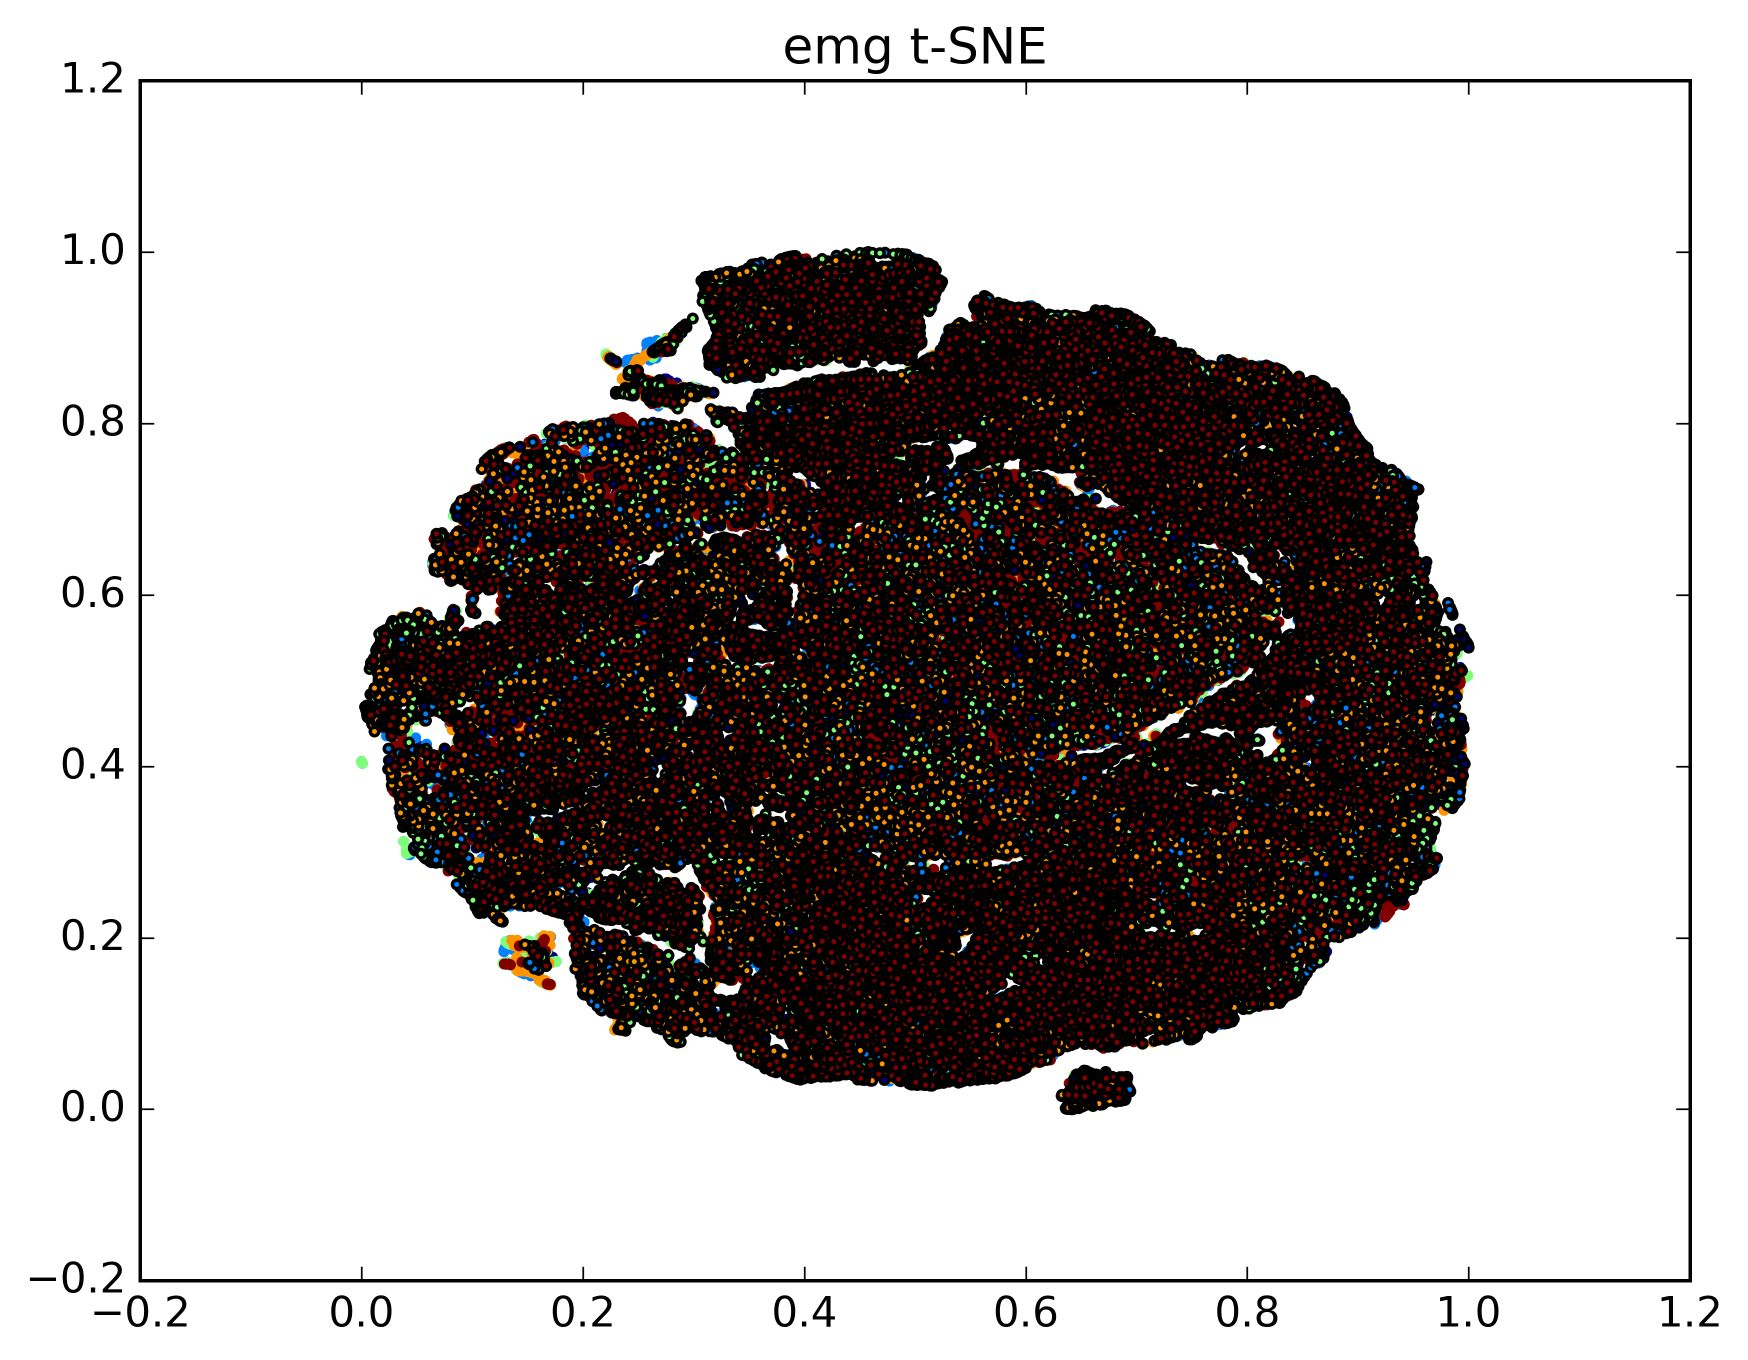
\includegraphics[width=1.0\textwidth]{emg.jpg}
	\caption{t-SNE plot for EMG data}
	\label{fig:emg}
\end{figure}


\subsection{Using a reference dataset}
The best way to check for generally plausible results seemed to create a reference dataset that can be used in the exact same way as the EEG and the EMG data respectively. Thus, the Matlab file \verb|WS_P1_S1.mat| was augmented to contain the additional datasets \verb|sp_static| and \verb|sp_var|:


\begin{itemize}	
	\item[sp\_static:]  A matrix of shape $3000\times32$ created for every window, i.e. trial. It contains randomly generated Gaussian values with same mean and variance. As thus all trials contain very similar values, a correctly working t-SNE implementation should create a plot showing all data points grouped together without any apparent structure.
	\item[sp\_var:]  A matrix of the same shape and size as \verb|sp_static|. Again, values are Gaussian with the same variance. However, this time the mean is changed for every trial, e.g. values for trial 1 have a mean of 10, values for trial 2 have a mean of 20, etc. In this case a functioning t-SNE implementation should output a plot showing a grouping of states within each trial while different trials should be separated from each other.
\end{itemize}


\begin{figure}
	\centering
	\begin{minipage}{0.5\textwidth}
		\centering
		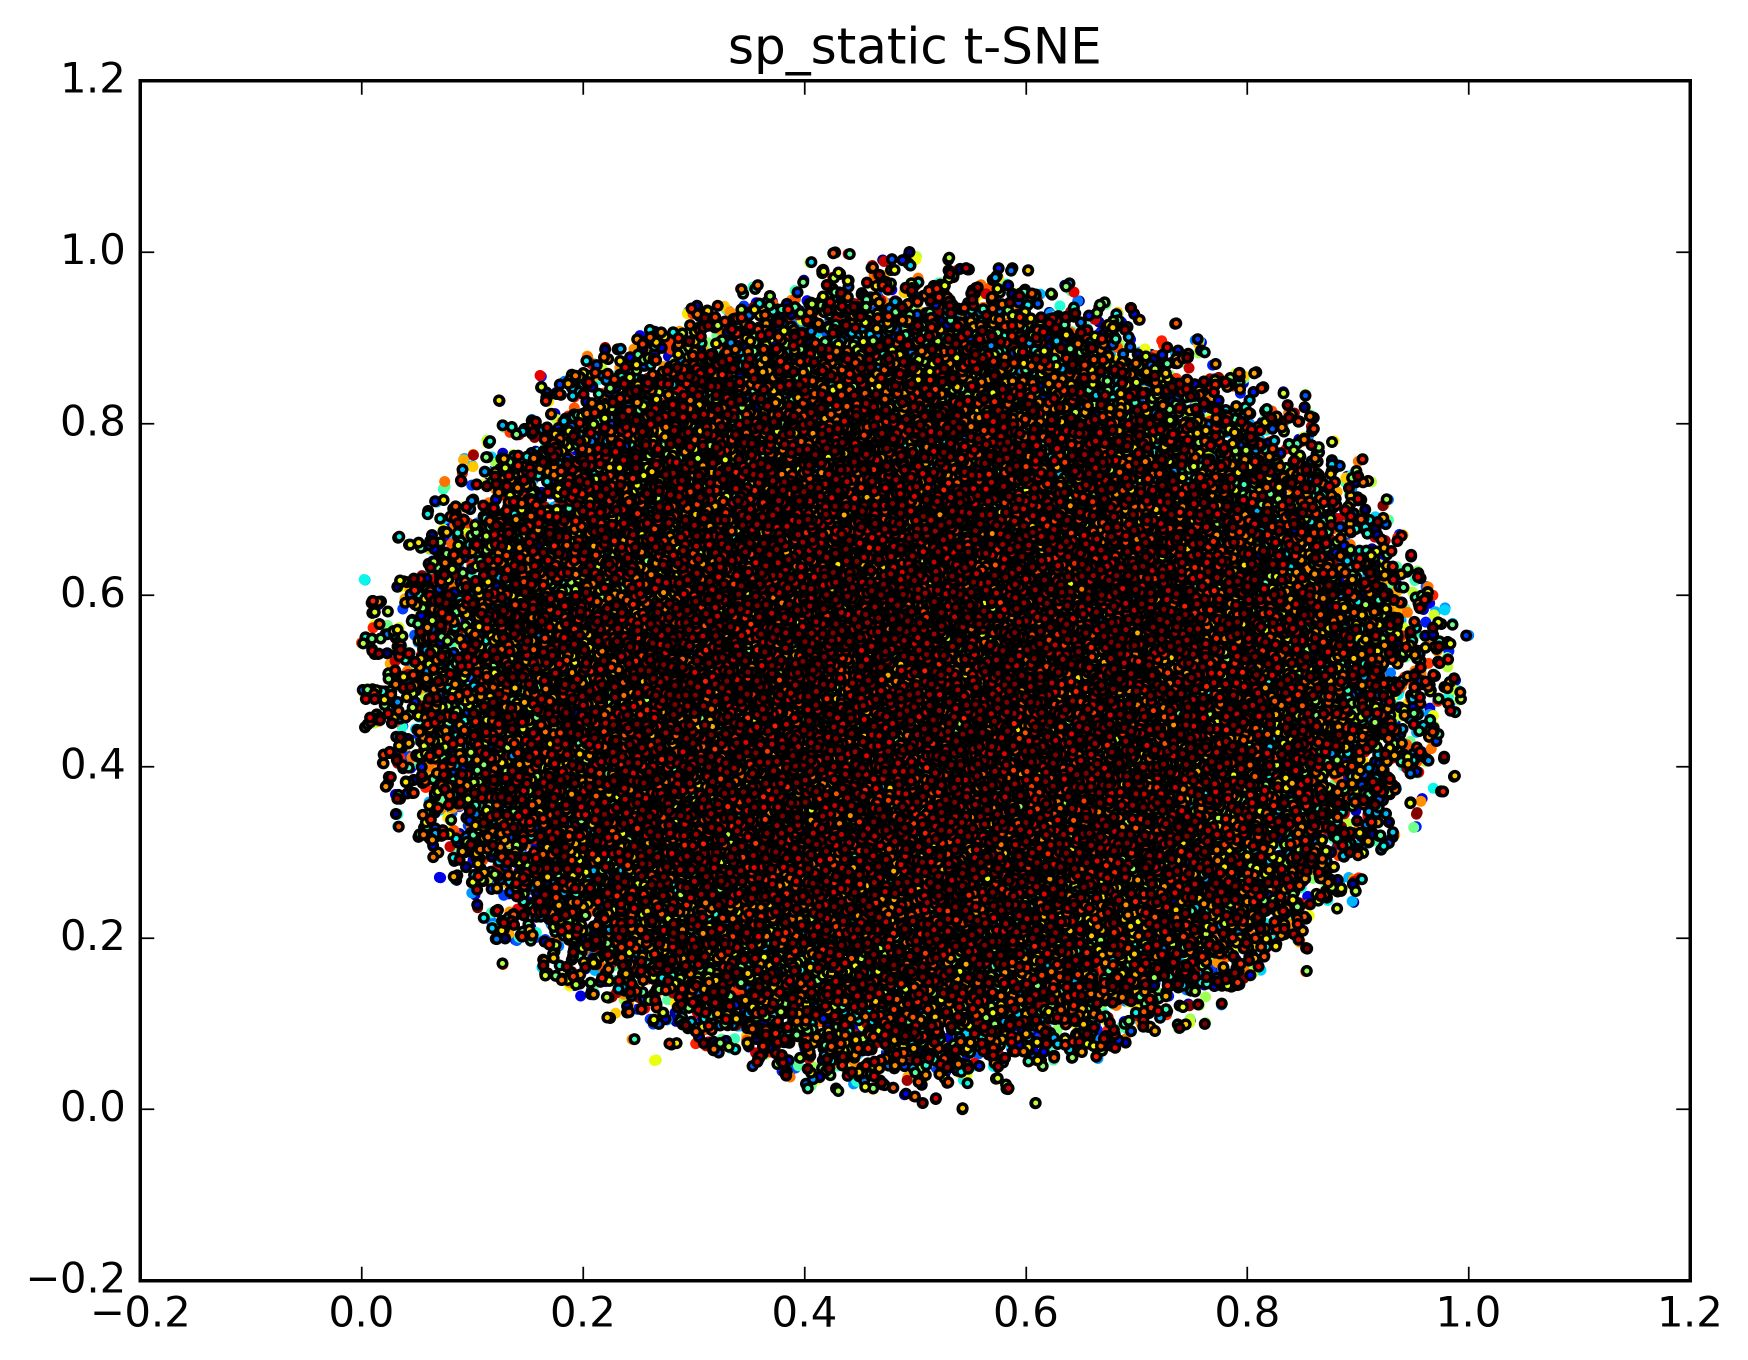
\includegraphics[width=1.0\textwidth]{sp_static.jpg}
		\caption{t-SNE on sp\_static}
		\label{fig:sp_static}
	\end{minipage}\hfill
	\begin{minipage}{0.5\textwidth}
		\centering
		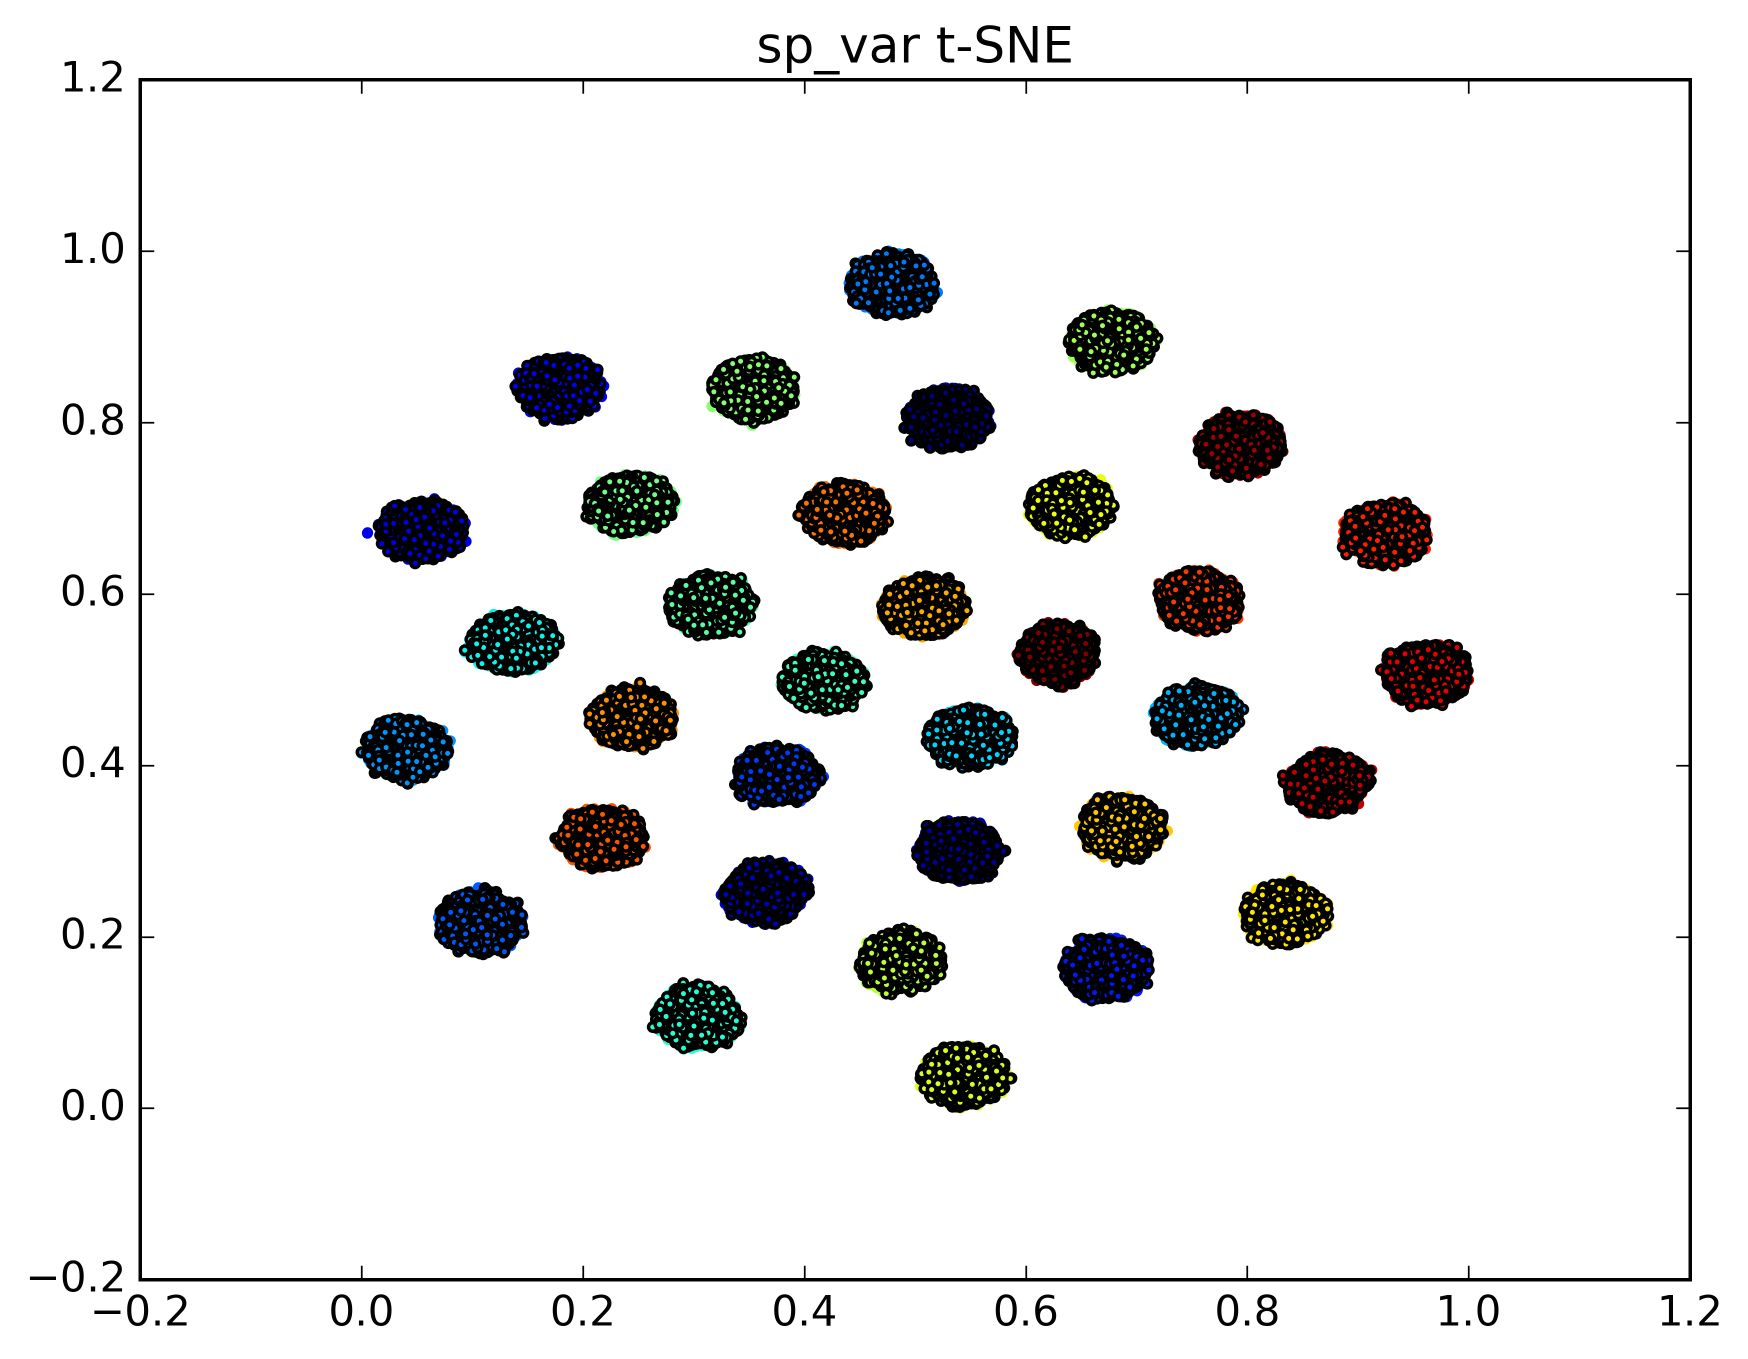
\includegraphics[width=1.0\textwidth]{sp_var.jpg}
		\caption{t-SNE on sp\_var}
		\label{fig:sp_var}
	\end{minipage}
\end{figure}

Figure \ref{fig:sp_static} and figure \ref{fig:sp_var} show the plots for \verb|sp_static| and \verb|sp_var| respectively. Both results look the way one would expect for the given data.
It should be noted that between the t-SNE runs on different datasets the code does not need to be altered except for a single line. In fact, figures \ref{fig:sp_static}, \ref{fig:sp_var} and \ref{fig:eeg} for \verb|sp_static|, \verb|sp_var| and \verb|eeg| were produced in this exact order by merely replacing the line \verb|datatype = 'sp_static'| with \verb|datatype = 'sp_var'| and \verb|datatype = 'eeg'| respectively.




\section{Further analysis}
If there is indeed some truth to the EEG plot in figure \ref{fig:eeg}, then it should be somewhat possible to classify the various trials using sample vectors as input. Thus, a Feedforward Neural Net was created. For this, an implementation was used that had been already applied successfully on the MNIST dataset multiple times, achieving a test error of about $1.6\%$. The script was altered just enough to allow application on the EEG data. In particular, the number of input and output neurons had to be changed. The EEG data containing 146982 samples in total was partitioned into a training-, validation- and test-set containing $4/9$, $2/9$ and $1/3$ of the original samples respectively.
The neural net was set up as follows:
\begin{itemize}
	\item Hidden Layer: 1
	\item Input neurons: 32
	\item Hidden neurons: 300
	\item Output neurons: 34
	\item Activation function: Sigmoid
	\item Optimizer: RmsProp
\end{itemize}
With these settings a validation error of $19.94\%$ and a test error of $19.69\%$ was achieved. Granted, this is not too great. However, considering that pure guessing should lead to an error of $97.06\%$ the neural net must have indeed found some pattern in the data corresponding to the individual trials. Figure \ref{fig:nnerror} shows the resulting error curves of the classification experiment. For comparison, the neural net was also applied on the EMG data using identical settings. The test error would in this case only reach $96.82\%$, which almost equals the expected error rate of sheer guessing, meaning there was no pattern to be found.

\begin{figure}[h]
	\centering
	\hspace*{-1.7cm}
	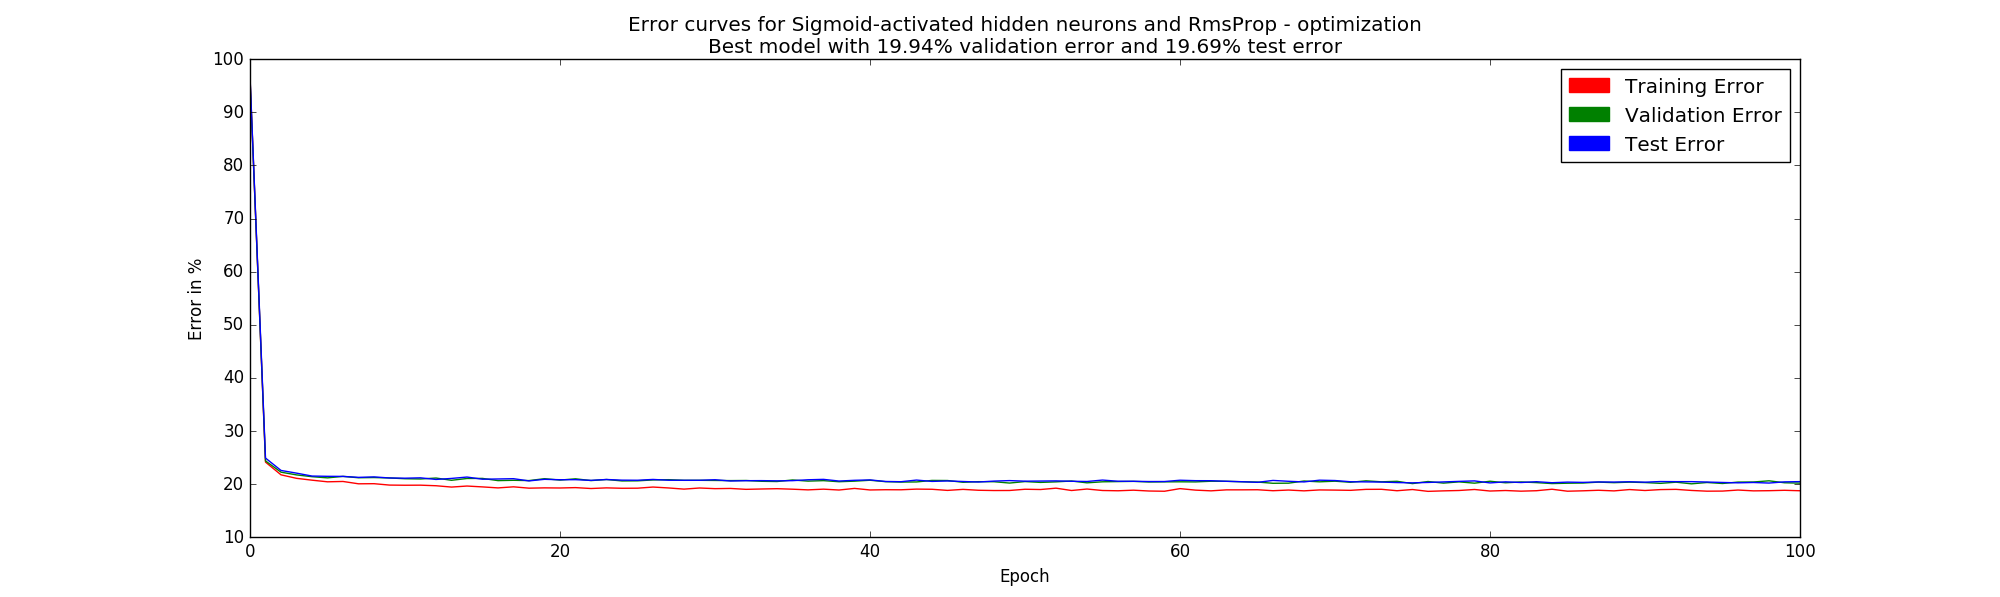
\includegraphics[width=1.24\textwidth]{nnerror.png}
	\caption{Error curves for classifying trials using a Feedforward Neural Net on the EEG data}
	\label{fig:nnerror}
\end{figure}




\section{Conclusion}
\emph{Participant 1} clearly was on an intense emotional rollercoaster during the course of the conducted lifting experiments, augmenting his mental state per trial. He obviously went through the 5 stages of emotional investment in scientific experiments as illustrated in figure \ref{fig:stickman}: Starting with highest euphoria for being part of great scientific research, followed by boredom for just holding a block repeatedly, then anger and major depression when asking himself what he is doing with his life. Finally he reached acceptance when he just gave in.

\begin{figure}[h]
	\centering
	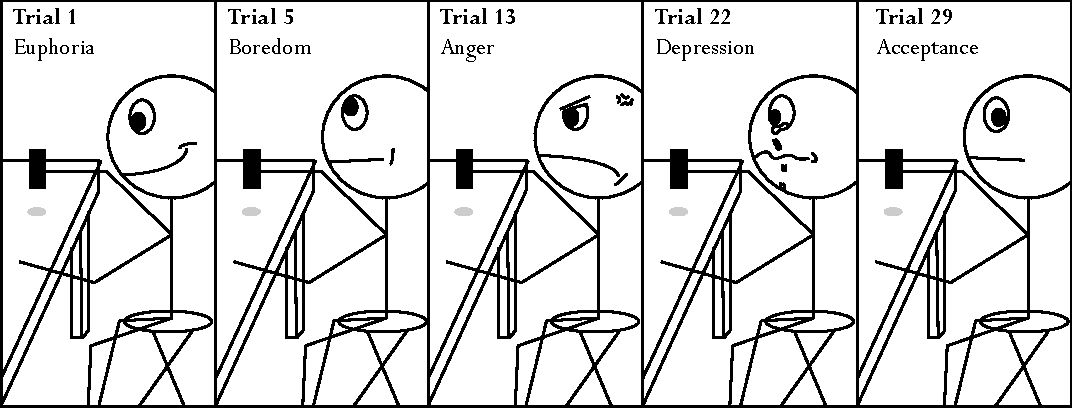
\includegraphics[width=1.0\textwidth]{stickman.pdf}
	\caption{Participant 1 going through 5 stages of emotional investment}
	\label{fig:stickman}
\end{figure}

Then again, maybe the findings about the EEG data are not that surprising after all. At last, the individual trials in one series are performed under varying conditions. In particular, inbetween the trials the used surface was changed unpredictably as well as the weight, the candidate had to lift. In the specific case of \emph{Participant 1}, \emph{Series 1} however, the surface did not change but was 'sandpaper' for all trials. The used weight on the other hand did change. Three different ones were in use: 165g, 330g and 660g. This might certainly have an effect on how the candidate perceives the trial and thus augment his mental state. And yet, if this was the deciding factor, one would expect a t-SNE plot with rather three major clusters grouping together trials for the various weights respectively. Plus, one might also, or maybe even more so, expect to see this being reflected in the EMG t-SNE plot.

How the varying conditions influence the EEG data will have to be examined more thoroughly. Furthermore, until now only the data of \emph{Participant 1}, \emph{Series 1} has been investigated in the presented manner. Other participants and series should be analyzed to see if their data shows similar characteristics.
Moreover, data had not been normalized before feeding neither to t-SNE nor the neural net. The effect of normalization on the EEG data will have to be examined, too.

\end{document}